\documentclass[]{article}
\usepackage{lmodern}
\usepackage{amssymb,amsmath}
\usepackage{ifxetex,ifluatex}
\usepackage{fixltx2e} % provides \textsubscript
\ifnum 0\ifxetex 1\fi\ifluatex 1\fi=0 % if pdftex
  \usepackage[T1]{fontenc}
  \usepackage[utf8]{inputenc}
\else % if luatex or xelatex
  \ifxetex
    \usepackage{mathspec}
  \else
    \usepackage{fontspec}
  \fi
  \defaultfontfeatures{Ligatures=TeX,Scale=MatchLowercase}
\fi
% use upquote if available, for straight quotes in verbatim environments
\IfFileExists{upquote.sty}{\usepackage{upquote}}{}
% use microtype if available
\IfFileExists{microtype.sty}{%
\usepackage{microtype}
\UseMicrotypeSet[protrusion]{basicmath} % disable protrusion for tt fonts
}{}
\usepackage[margin=1in]{geometry}
\usepackage{hyperref}
\hypersetup{unicode=true,
            pdftitle={Project 2},
            pdfborder={0 0 0},
            breaklinks=true}
\urlstyle{same}  % don't use monospace font for urls
\usepackage{longtable,booktabs}
\usepackage{graphicx,grffile}
\makeatletter
\def\maxwidth{\ifdim\Gin@nat@width>\linewidth\linewidth\else\Gin@nat@width\fi}
\def\maxheight{\ifdim\Gin@nat@height>\textheight\textheight\else\Gin@nat@height\fi}
\makeatother
% Scale images if necessary, so that they will not overflow the page
% margins by default, and it is still possible to overwrite the defaults
% using explicit options in \includegraphics[width, height, ...]{}
\setkeys{Gin}{width=\maxwidth,height=\maxheight,keepaspectratio}
\IfFileExists{parskip.sty}{%
\usepackage{parskip}
}{% else
\setlength{\parindent}{0pt}
\setlength{\parskip}{6pt plus 2pt minus 1pt}
}
\setlength{\emergencystretch}{3em}  % prevent overfull lines
\providecommand{\tightlist}{%
  \setlength{\itemsep}{0pt}\setlength{\parskip}{0pt}}
\setcounter{secnumdepth}{0}
% Redefines (sub)paragraphs to behave more like sections
\ifx\paragraph\undefined\else
\let\oldparagraph\paragraph
\renewcommand{\paragraph}[1]{\oldparagraph{#1}\mbox{}}
\fi
\ifx\subparagraph\undefined\else
\let\oldsubparagraph\subparagraph
\renewcommand{\subparagraph}[1]{\oldsubparagraph{#1}\mbox{}}
\fi

%%% Use protect on footnotes to avoid problems with footnotes in titles
\let\rmarkdownfootnote\footnote%
\def\footnote{\protect\rmarkdownfootnote}

%%% Change title format to be more compact
\usepackage{titling}

% Create subtitle command for use in maketitle
\newcommand{\subtitle}[1]{
  \posttitle{
    \begin{center}\large#1\end{center}
    }
}

\setlength{\droptitle}{-2em}
  \title{Project 2}
  \pretitle{\vspace{\droptitle}\centering\huge}
  \posttitle{\par}
  \author{}
  \preauthor{}\postauthor{}
  \date{}
  \predate{}\postdate{}


\begin{document}
\maketitle

\section{Introduction}\label{introduction}

This is Project 2 for STAT 557 2018 Spring by Meridith Bartley and Fei
Jiang. The aim of this project is to practice the k-means algorithm and
the k-nearest neighbor algorithm. In this project we applied both
algorithms to seed data in order to classify/cluster by seed type.

\section{Description of Data}\label{description-of-data}

The examined group comprised kernels belonging to three different
varieties of wheat: Kama, Rosa and Canadian, 70 elements each, randomly
selected for the experiment. High quality visualization of the internal
kernel structure was detected using a soft X-ray technique. It is
non-destructive and considerably cheaper than other more sophisticated
imaging techniques like scanning microscopy or laser technology. The
images were recorded on 13x18 cm X-ray KODAK plates. Studies were
conducted using combine harvested wheat grain originating from
experimental fields, explored at the Institute of Agrophysics of the
Polish Academy of Sciences in Lublin.

Boxplots for each attribute used as explanitory variables in the
subsequent classification models are included below. This EDA allows for
early indication of which variables may possibly be ommitted during
dimention reduction. That is, what properties do not differ
significantly between seed types.

\subsection{Exploritory Data Analysis}\label{exploritory-data-analysis}

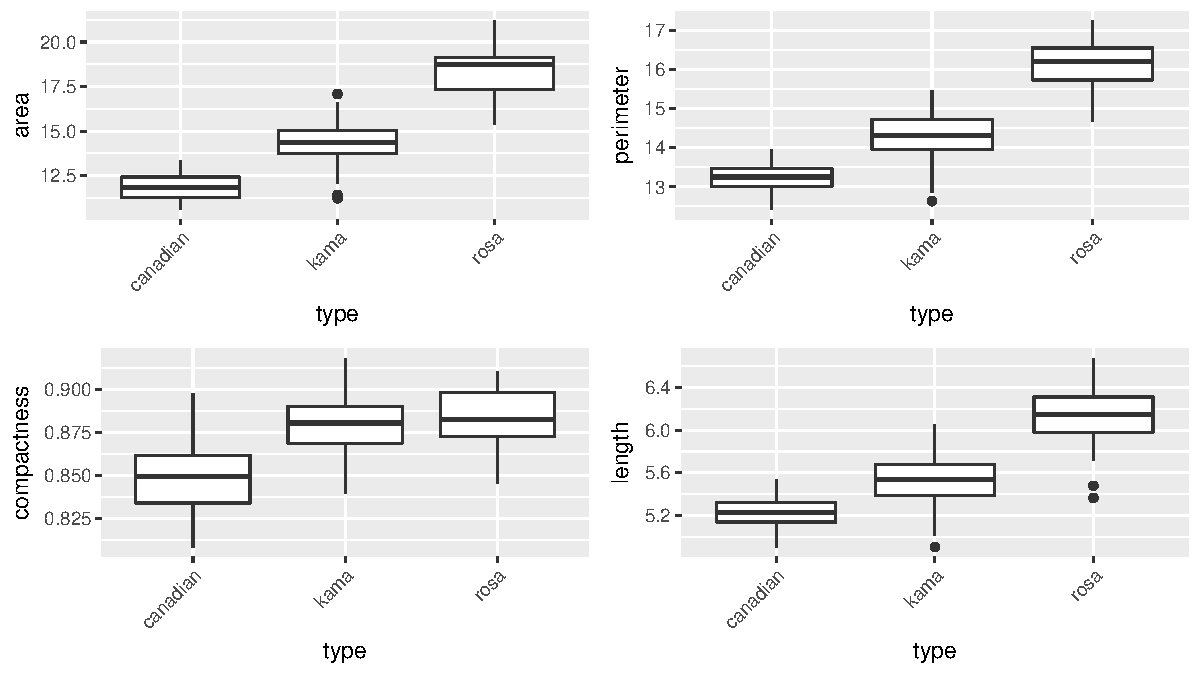
\includegraphics{Project2_files/figure-latex/EDA - Mer-1.pdf}
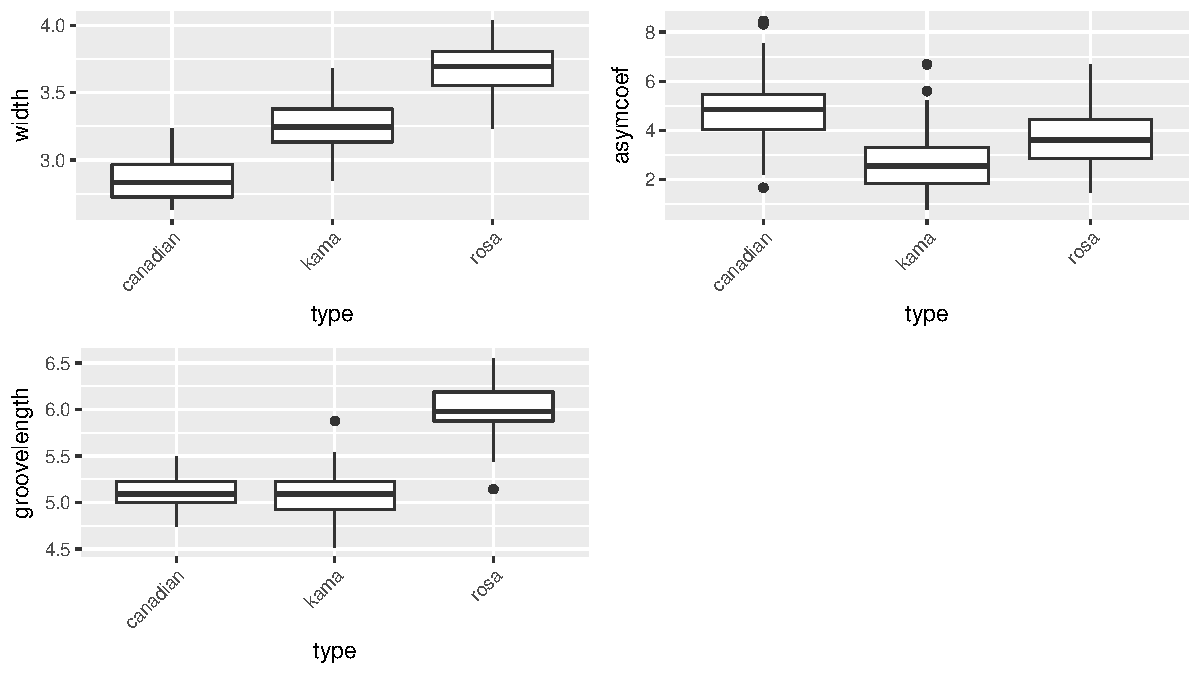
\includegraphics{Project2_files/figure-latex/EDA - Mer-2.pdf}
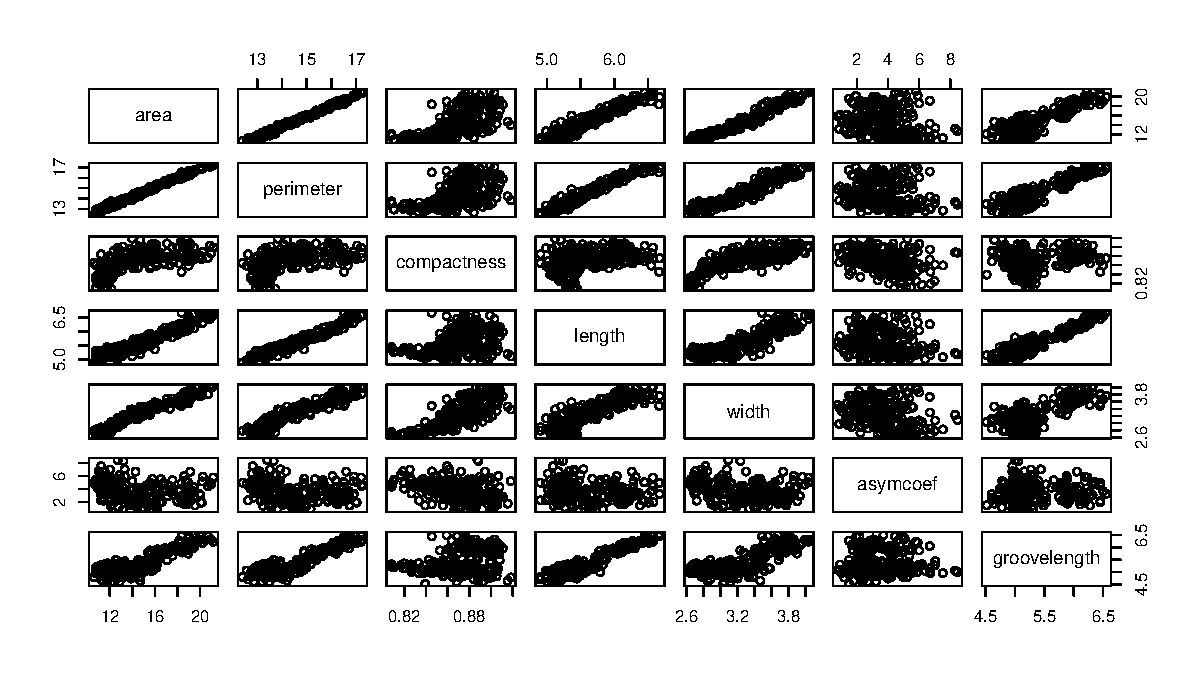
\includegraphics{Project2_files/figure-latex/EDA - Mer-3.pdf}

\section{Principle Component
Analysis}\label{principle-component-analysis}

In order to test whether dimension reduction will improve predictions we
also conducted Principle Component Analysis on the original dataset to
get a new dataset with fewer dimensions. According to our PCA results,
the first two component in total can explain about 99.302\% of variance
of the original database. The coefficients of the relevent componets are
listed in the table below. Therefore, we took the first two components
and the seed type values to build a new dataset with less dimensions.

\begin{longtable}[]{@{}lrrrrrrr@{}}
\toprule
& PC1 & PC2 & PC3 & PC4 & PC5 & PC6 & PC7\tabularnewline
\midrule
\endhead
Standard deviation & 3.28532 & 1.459265 & 0.2713485 & 0.1135231 &
0.0524235 & 0.0396289 & 0.0054457\tabularnewline
Proportion of Variance & 0.82939 & 0.163630 & 0.0056600 & 0.0009900 &
0.0002100 & 0.0001200 & 0.0000000\tabularnewline
Cumulative Proportion & 0.82939 & 0.993020 & 0.9986800 & 0.9996700 &
0.9998800 & 1.0000000 & 1.0000000\tabularnewline
\bottomrule
\end{longtable}

\begin{longtable}[]{@{}lrr@{}}
\toprule
& PC1 & PC2\tabularnewline
\midrule
\endhead
area & 0.8842285 & 0.1008058\tabularnewline
perimeter & 0.3954054 & 0.0564896\tabularnewline
compactness & 0.0043113 & -0.0028947\tabularnewline
length & 0.1285445 & 0.0306217\tabularnewline
width & 0.1110591 & 0.0023723\tabularnewline
asymcoef & -0.1276156 & 0.9894105\tabularnewline
groovelength & 0.1289665 & 0.0822334\tabularnewline
\bottomrule
\end{longtable}

\section{Analysis}\label{analysis}

In the following analysis with two methods (k means and k-nearest
neighbor algorithms - both supervised and unsupervised) and two datasets
(original and dimension-reduced), we randomly selected 80\% of the
entire data as training data and the rest 20\% as test data.

\subsection{K-Means Algorithm - Unsupervised clustering of Original
Dataset}\label{k-means-algorithm---unsupervised-clustering-of-original-dataset}

When conducting the k-means algorthm with on the original dataset and
found that the overall prediction accuracy of our model in testing data
is about 90\%. In addition, we applied the k-means algorithem to a
dimension reduced data set using the first two principal compoents and
found that with the testing data there was about 90\% accuracy. In the
following plot we can see the cluster plot that uses PCA to draw the
data using the first two principal components to explain the data.

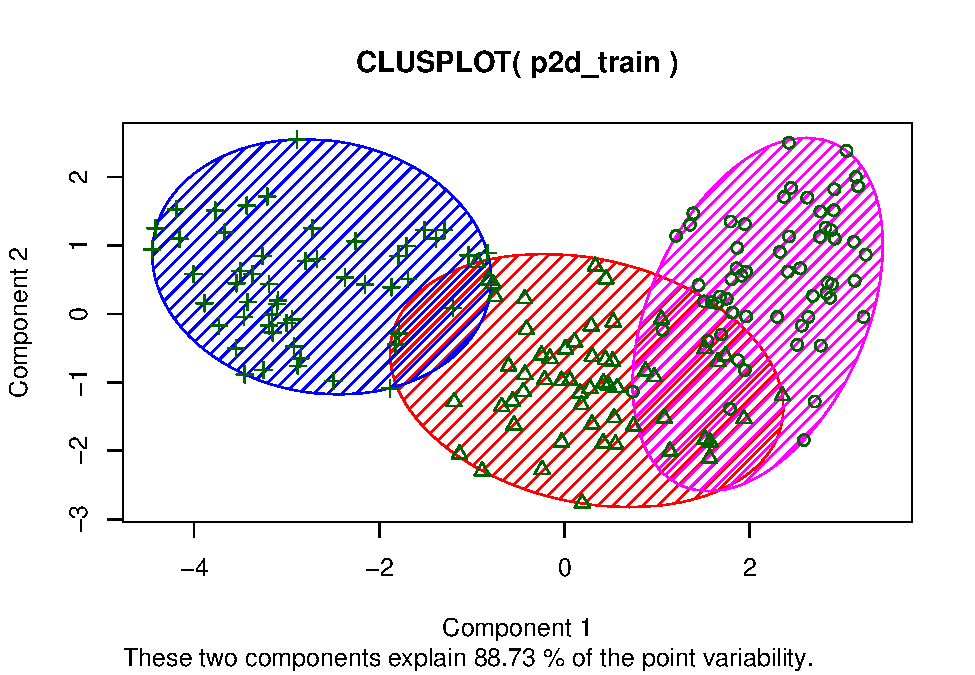
\includegraphics{Project2_files/figure-latex/unnamed-chunk-3-1.pdf}

While we have reported the outcomes for k = 3, we also explored the
possibilities of other size selections for k (see below table for
comparison of accuracies). We also looked at total Within Groups Sums of
Squares as a measure of how well our clusters fit the data. This is a
measure of the distance the vectors in each cluster are from their
respected centroid.The goal is to minimiza this value but no further
than when the rate of improvement drops off. The scree plot below of
these WSS values do indicate that is an appropraite number of clusters
to choose. Indeed we do know from the data available that there are
three seed types included.

\begin{longtable}[]{@{}rr@{}}
\toprule
K & \% Accuracy\tabularnewline
\midrule
\endhead
2 & 98\tabularnewline
3 & 90\tabularnewline
4 & 90\tabularnewline
5 & 83\tabularnewline
6 & 93\tabularnewline
7 & 57\tabularnewline
8 & 88\tabularnewline
9 & 95\tabularnewline
10 & 40\tabularnewline
\bottomrule
\end{longtable}

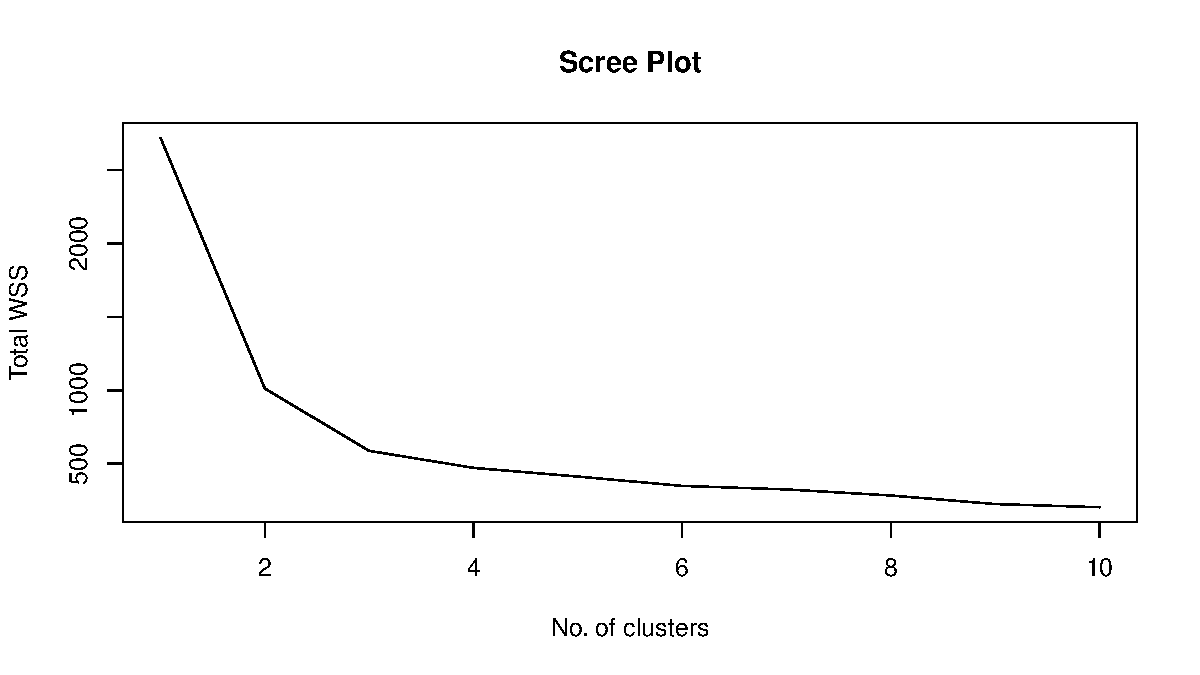
\includegraphics{Project2_files/figure-latex/unnamed-chunk-5-1.pdf}

\subsection{K-Nearest Neighbor - Supervised clustering in Original
Dataset}\label{k-nearest-neighbor---supervised-clustering-in-original-dataset}

In this section, supervised K-nearest clustering is applied in the
original dataset. The true and predictied lables in training and test
data are shown in the figures below. In those figures, only first two
predictors were shown. In general, in the training data, we obtained the
accuracy rate of 92.9\% and in the testing data, the accuarcy rate is
about 90.5\%. We think we reached a satisfying accuracy rate.

In the following plots we explore the true labels compared to those
predicted by K-nearest neighbor clustering. We do this for both the
original training and testing datasets. Not that we have plotted the
data by area and the asymmetrical coefficent. It's clear that this
method of clusing the data is performing well.

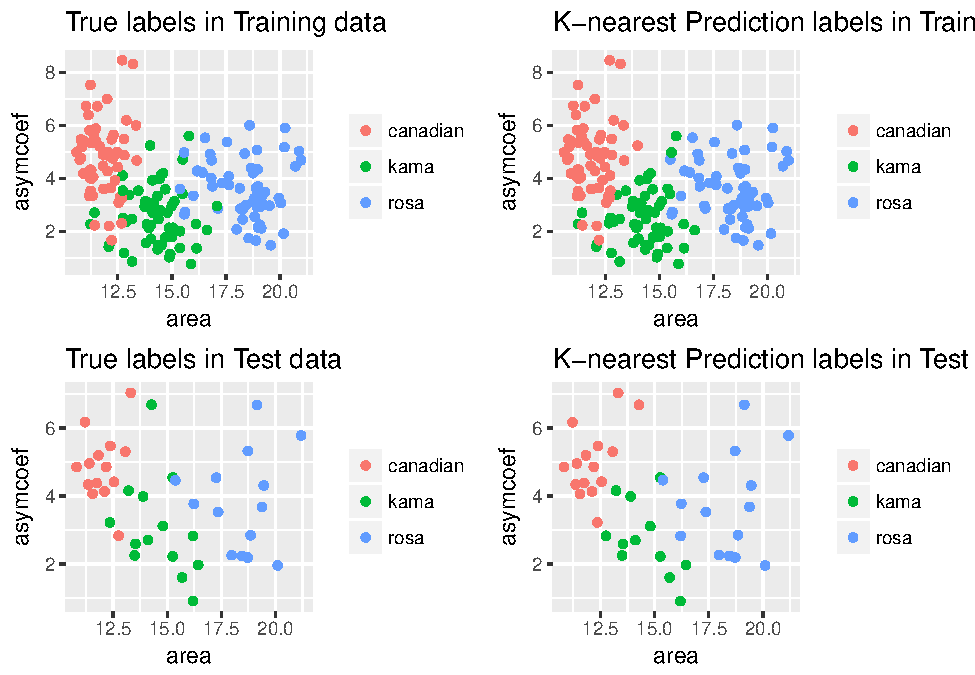
\includegraphics{Project2_files/figure-latex/- Fei-1.pdf}

\subsection{K-Means and K-Centers Algorithm - Unsupervised clustering in
Reduced Dataset (First Two Principle
Components)}\label{k-means-and-k-centers-algorithm---unsupervised-clustering-in-reduced-dataset-first-two-principle-components}

In this section, we applied unsupervised K-Means and K-Centers
clustering algorithms to the reduced dataset (first two principle
components).We tried 9 different numbers of clusters: 2 to 10 and
plotted the scatter plot for each cluster number and for each algorithm.
As the below figures show, there are differences between K-Center and
K-Means clustering results. That is because k-means focuses on average
distance while k-center focuses on worst scenario.

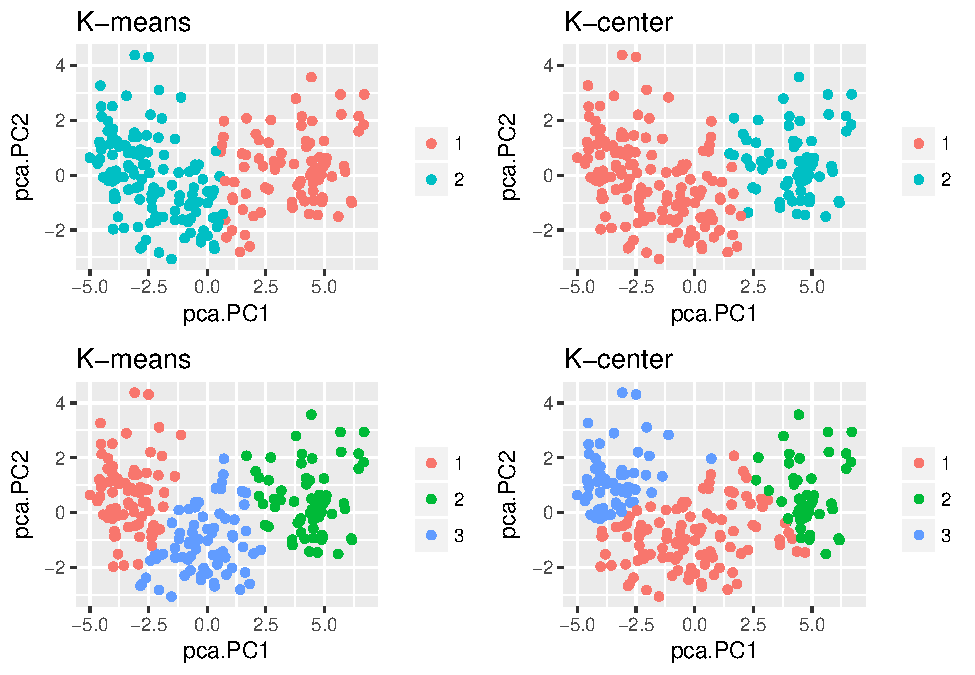
\includegraphics{Project2_files/figure-latex/unnamed-chunk-6-1.pdf}
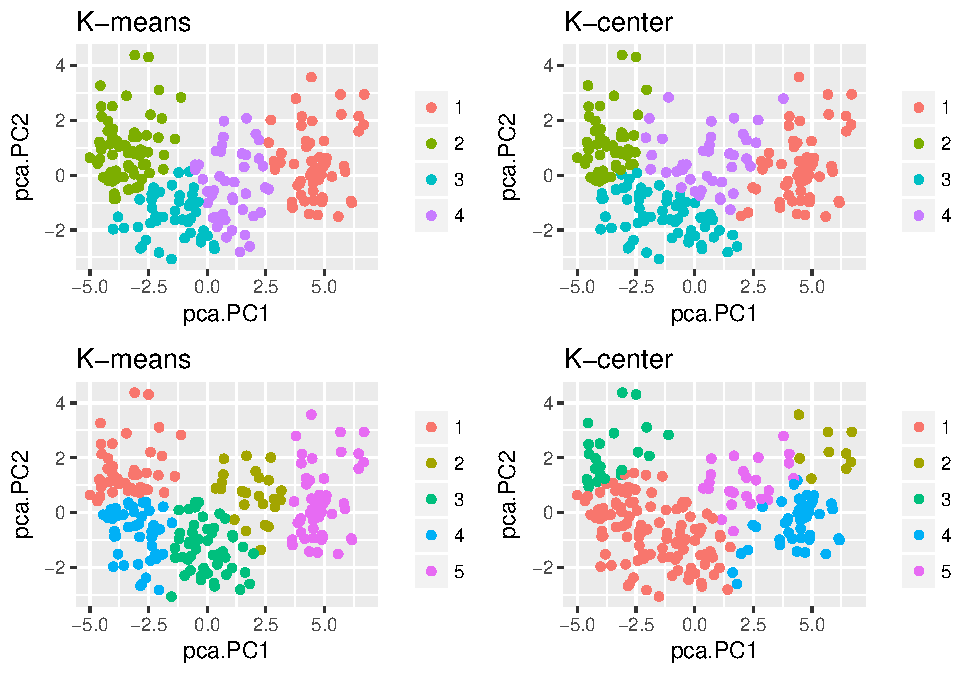
\includegraphics{Project2_files/figure-latex/unnamed-chunk-6-2.pdf}
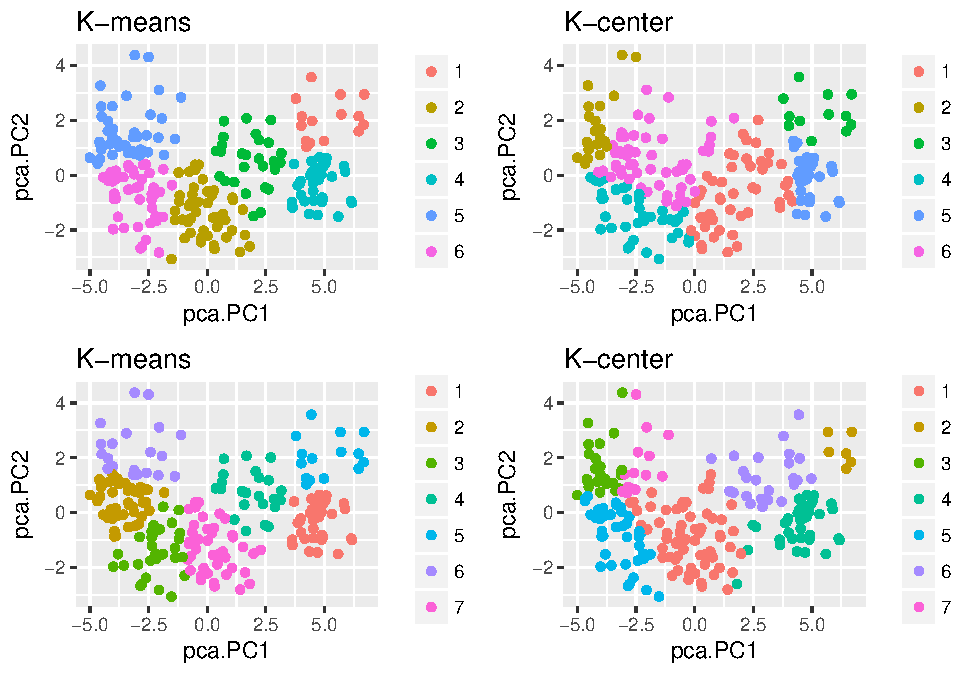
\includegraphics{Project2_files/figure-latex/unnamed-chunk-6-3.pdf}
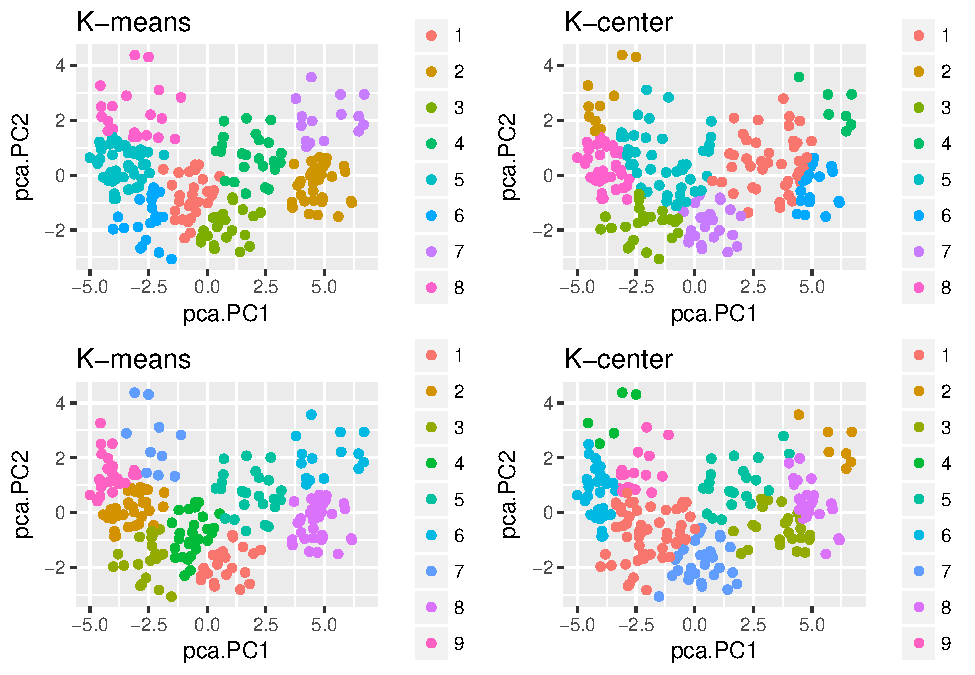
\includegraphics{Project2_files/figure-latex/unnamed-chunk-6-4.pdf}
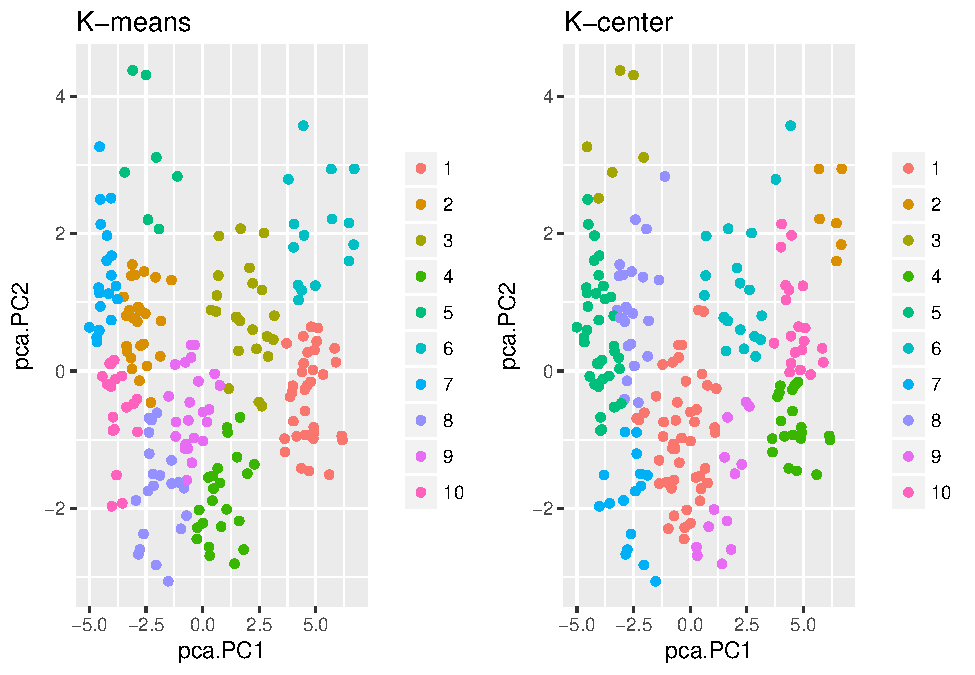
\includegraphics{Project2_files/figure-latex/unnamed-chunk-6-5.pdf}

\section{Conclusions}\label{conclusions}

To sum up, we finisehd the following analysis in this project.

\begin{itemize}
\item
  The K-means clustering method on both the original and dimension
  reduced training and testing data, both showing similar accuracies of
  about 90\% for the testing data.
\item
  Confirmed a cluster size of by examining the Within Sums of Squares
  values.
\item
  The supervised K-nearest clustering method achieved over 90\% accuracy
  in both training and test data, which is satisfying.
\item
  Applying differet k values, we explored the contrasting difference
  between k-means and k-center clustering methods.
\end{itemize}

\section{Contributions}\label{contributions}

The different tasks required to complete this project were equally
divided between Meridith and Fei. K-means and cross-valiation analyses
were completed by Meridith while Fei was responsible for K-nearest and
K-center comparison. Both members of this group contributed to this
report.


\end{document}
